\documentclass[12pt,letter]{article}
\usepackage[moduleName=Terracillator]{KautenjaDSP}
% import a debugging package to show the margin boxes
% \usepackage{showframe}
% set the graphics path to the img directory
\graphicspath{{img/}}

% algorithm2e stuff
% \SetKwInOut{Objects}{$\CKmatrix{O}$}
% \SetKwInOut{Weights}{$\CKvector{w}$}

\begin{document}
\titlePage{Terracillator-Logo}{Terracillator-Module}{KautenjaDSP}

% -------------------
% MARK: Overview
% -------------------

\section{Overview}

2A03 is an emulation of the 2A03 sound chip from the Nintendo Entertainment System (NES) for VCV Rack. The 2A03 chip contains two pulse wave generators, a quantized triangle wave generator, and a noise generator. The original chip featured a DMC loader for playing samples that has been omitted in this emulation.

2A03 provides the key features of the 2A03 chip, namely,
\begin{itemize}
  \item \textbf{Dual pulse wave generator:} Dual 8-bit pulse waves with four duty cycles: $12.5\%$, $25\%$, $50\%$, and $75\%$;
  \item \textbf{Quantized triangle wave generator:} Generate NES style triangle wave with 16 steps of quantization;
  \item \textbf{Noise generator:} generate pseudo-random numbers at 16 different frequencies; and
  \item \textbf{Linear Feedback Shift Register (LFSR):} for that old-school 8-bit randomness!
\end{itemize}

% -------------------
% MARK: Panel Layout
% -------------------

\clearpage
\section{Panel Layout}

\begin{figure}[!htp]
\centering
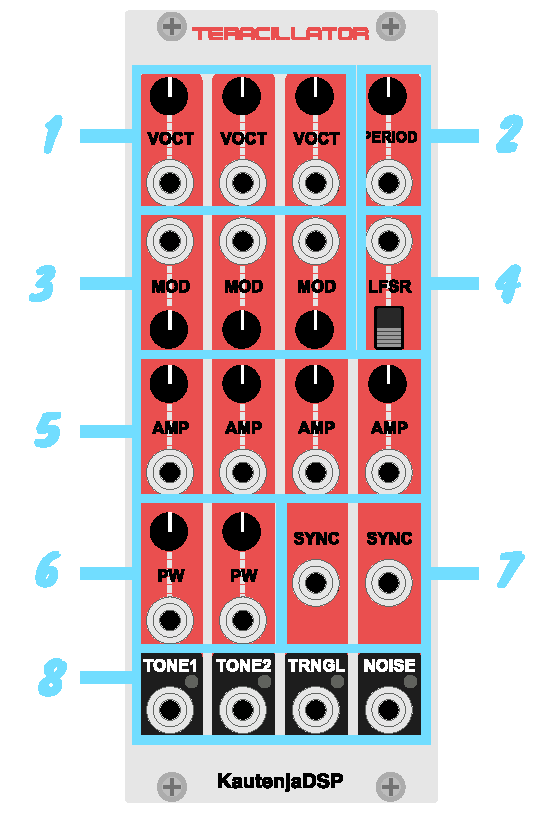
\includegraphics{Terracillator-Manual}
\end{figure}

\begin{enumerate}
  \item Coarse frequency control over the four oscillators.
  \item $V$/Octave inputs for pulse1, pulse2, and triangle waveform generators.
  \item linear CV frequency modulation for pulse1, pulse2, and triangle waveform generators.
  \item Pulse width selector. Chooses between four duty cycles: $12.5\%$, $25\%$, $50\%$, and $75\%$.
  \item CV LFSR gate, high at $2V$. Holds the LFSR generator as long as the input voltage is $>2V$.
  \item Period of randomness $\in [0, 15]$ for the noise generator. See Table~\ref{tab:noise-periods} for a mapping from period to sample rate, frequency, and MIDI note.
  \item Coarse amplitude control over the oscillators using the 4-bit amplifier. When no input is connected, the slider controls the level from $0\%$ to $100\%$. When an input is connected, the slider acts as an attenuator.
  \item Channel outputs, ${\approx}10V_{pp}$.
\end{enumerate}

\begin{table}[!htp]
\centering
\caption{Mapping of noise period to sample rate, fundamental frequency, and MIDI note.}
\label{tab:noise-periods}
\begin{tabular}{|l||r|r|r|}
\hline
 Period  & Sample rate   & Fundamental   & MIDI note \\
\hline\hline
 0       & $447443.2 Hz$ & $4811.2 Hz$   & 110.41    \\
 1       & $223721.6 Hz$ & $2405.6 Hz$   & 98.41     \\
 2       & $111860.8 Hz$ & $1202.8 Hz$   & 86.41     \\
 3       & $55930.4 Hz$  & $601.4 Hz$    & 74.41     \\
 4       & $27965.2 Hz$  & $300.7 Hz$    & 62.41     \\
 5       & $18643.5 Hz$  & $200.5 Hz$    & 55.39     \\
 6       & $13982.6 Hz$  & $150.4 Hz$    & 50.41     \\
 7       & $11186.1 Hz$  & $120.3 Hz$    & 46.55     \\
 8       & $8860.3 Hz$   & $95.3 Hz$     & 42.51     \\
 9       & $7046.3 Hz$   & $75.8 Hz$     & 38.55     \\
 10      & $4709.9 Hz$   & $50.6 Hz$     & 31.57     \\
 11      & $3523.2 Hz$   & $37.9 Hz$     & 26.55     \\
 12      & $2348.8 Hz$   & $25.3 Hz$     & 19.53     \\
 13      & $1761.6 Hz$   & $18.9 Hz$     & 14.55     \\
 14      & $879.9 Hz$    & $9.5 Hz$      & 2.53      \\
 15      & $440.0 Hz$    & $4.7 Hz$      & -9.47     \\
\hline
\end{tabular}
\end{table}

% -------------------
% MARK: References
% -------------------

\clearpage
\renewcommand\refname{References \& Acknowledgments}
\nocite{*}
\bibliographystyle{apalike}
\bibliography{references}

\end{document}
